\chapter{Proof of Concept}
\label{chapter:poc}

    This last chapter will deal with a proof-of-concept (PoC) project that was realized during this work. We will fill the abstract components of the reference architecture from \autoref{chapter:architecture-proposal} with concrete technologies and apply them to a setting that mimics a real-world scenario, while also exploring and comparing which technologies might be best suited for different use cases. In the project, we focused on the provisioning of infrastructure, since it is the most challenging part of realizing such an IIoT system. The resources and the cloud subscription used in this proof-of-concept were provided by MaibornWolff GmbH.

    \section{Provisioning the Infrastructure}

        In this PoC we wanted to set up each environment, i.e.\ edge, fog and cloud, that was introduced in the reference architecture. For the edge environment, a \textit{Supermicro SMC X10 A1SAi-2750F} server, which provides an IPMI and supports PXE boot (see \autoref{subsection:network-boot}), was used, particularly to demonstrate how bare-metal machines can be provisioned. In this project, we have decided against virtualization (see \autoref{section:virtualization}) and sticked to deploying directly to the bare-metal machines. The cloud environment was set up in the Microsoft Azure cloud, mainly revolving around their managed Kubernetes cluster ``Azure Kubernetes Service (AKS)''. Lastly, the fog environment was created on a pre-provisioned Ubuntu machine, which was already bootstrapped with the Kubernetes distribution ``Rancher K3s'' and a running instance of ClusterAPI. As discussed in \autoref{subsection:capi}, we used ClusterAPI to provision and manage the other Kubernetes instances in combination with infrastructure providers specific to the according infrastructure they should provision to. \newline
    
        For the cloud environment, we installed the official ClusterAPI Provider Azure (CAPZ) \cite{azure_capi_provider} as the infrastructure provider into our management cluster which supports managing Kubernetes clusters in the Microsoft Azure cloud. Using custom resource definitions in Kubernetes, we could provision and operate a workload Kubernetes cluster fully managed by the cloud provider by simply applying YAML-manifests into our management cluster. Using the ClusterAPI command line interface ``clusterctl'' we were able to generate these manifests, and only needed to adjust domain-specific configuration like the name of the cluster or the number of cluster nodes. \newline

        The more interesting environments in this PoC were those that required provisioning directly onto bare-metal infrastructure. The hardware used in this project supported PXE and IPMI, so using an according ClusterAPI infrastructure provider had to be chosen. For this purpose, we evaluated the following options:

        \begin{itemize}
            \item Canonical MAAS | Metal as a Service
            \item Tinkerbell
            \item Metal$^3$ (pronounced ``metal kubed'')
            \item Sidero Metal
        \end{itemize}

        \noindent Canonical MAAS is a tool that provides an abstraction over bare-metal provisioning and offers a rich API to the outside, which can be consumed by the ``Cluster API Provider for MAAS''. In practice, a dedicated machine hosts the MAAS instance and is responsible for the out-of-band management (see \autoref{subsection:network-boot}) of the target infrastructure. It achieves this by mainly building upon DHCP, IPMI, PXE and TFTP and offers a nice abstraction layer over these low-level protocols. MAAS also ships a user interface that helps in managing large-scale bare-metal clouds, custom OS images, disks and network configuration, authentication, RBAC configuration and many more useful features. The main drawback of using MAAS for provisioning the bare-metal infrastructure in this work however is that it necessitates the provisioning and operation of an additional machine specifically to host MAAS itself. This requirement adds complexity and overhead since it involves not only setting up another server but also ensuring its reliable operation and maintenance, which includes configuration and ongoing management tasks. Since our idea was to use Kubernetes as a uniform technology across all environments in order to only have to manage one technology, we decided not to use MAAS in this PoC and kept looking for a Kubernetes-native solution \cite{canonical_maas}. \newline

        A very promising project is Metal$^3$, which provides a set of tools for managing bare-metal infrastructure using Kubernetes. It consists of three components, that make the provisioning of bare-metal machines possible: the ``ClusterAPI Provider Metal$^3$'', the so-called ``Bare Metal Operator'' and the external tool ``OpenStack Ironic''. The ClusterAPI provider serves as the infrastructure provider and enables the creation and management of physical servers using custom resource definitions in Kubernetes. The Bare Metal Operator works in tandem with the ClusterAPI provider and is responsible for provisioning and managing the lifecycle of physical servers. It interacts with the underlying bare-metal management tool Ironic commonly known from the OpenStack project to perform tasks like provisioning, de\-pro\-vi\-sio\-ning, and updating the hardware. The Bare Metal Operator receives instructions from the ClusterAPI provider and acts upon these instructions to manage the physical hardware through Ironic. The robust tool Ironic again relies on technologies like IPMI and Redfish to manage the bare-metal machines. The Metal$^3$ project appears to be one of the most robust and reliable projects for managing bare-metal infrastructure from Kubernetes. Especially through its reliance on the battle-tested OpenStack component ``Ironic'' the project is capable of deploying to a broad variety of infrastructure and is a solid choice for large projects. The downside of Metal$^3$ however is, that it adds much complexity. Developers have to maintain their own instance of OpenStack Ironic and the Metal$^3$ Bare Metal Operator, which are both large and complex projects with setups that are far from trivial. It has to be evaluated on a project basis, whether the benefit of employing one of the most reliable projects for bare-metal management outweighs the downside of introducing high complexity into the system \cite{metal3_docs, metal3_bare_metal_operator}. Due to the simplicity of the PoC setup, we chose against adding this level of complexity into our system. \newline

        Another Kubernetes-native tool for provisioning and managing bare-metal infrastructure is ``Tinkerbell''. Apart from being a microservice-driven application, Tinkerbell operates similarly to Metal$^3$ with the difference of not relying on external tools but shipping its own, e.g. ``Boots'' as a DHCP server or ``PBnJ'' for out-of-bands management via the BMC (see \autoref{subsection:network-boot}) of bare-metal machines. However, since at the time of writing this work the ClusterAPI Provider Tinkerbell was still not ready for production use and only supported Kubernetes versions up to v1.22, which was marked as end-of-life for over 15 months now, we decided against the use of Tinkerbell for this PoC project \cite{tinkerbell}. \newline
        
        Finally, Sidero Metal was the last tool we evaluated. Similar to Metal$^3$ and Tinkerbell, it allows for Kubernetes-native bare-metal management using ClusterAPI. The project includes a metadata service, PXE and TFTP servers, as well as BMC and IPMI management for automation, which all come in handy in practice. Sidero Metal not only consists of a ClusterAPI infrastructure provider but also a bootstrap provider and a control plane provider. This means that Sidero Metal is not only managing the infrastructure itself but also provides an end-to-end ecosystem for deploying Kubernetes. Sidero Metal chooses ``Talos Linux'' as a secure, immutable, and minimal base operating system for Kubernetes nodes, which ensures a secure and robust basis for running Kubernetes in production. Overall the project shines through its simplicity and a feature set, that does exactly what was required in this PoC, which is the reason why Sidero Metal was chosen as the ClusterAPI provider for bare-metal management in this project \cite{siderometal, taloslinux}.\newline

        Generally, if a bare-metal management solution based on ClusterAPI is required, we can recommend using Canonical MAAS or if a Kubernetes-native solution is preferred Sidero Metal for smaller projects. In large-scale and productive systems, where reliability and robustness are key requirements, Metal$^3$ is a solid choice but requires more domain knowledge and setup.\newline

        \begin{figure}[htbp]
            \centering
            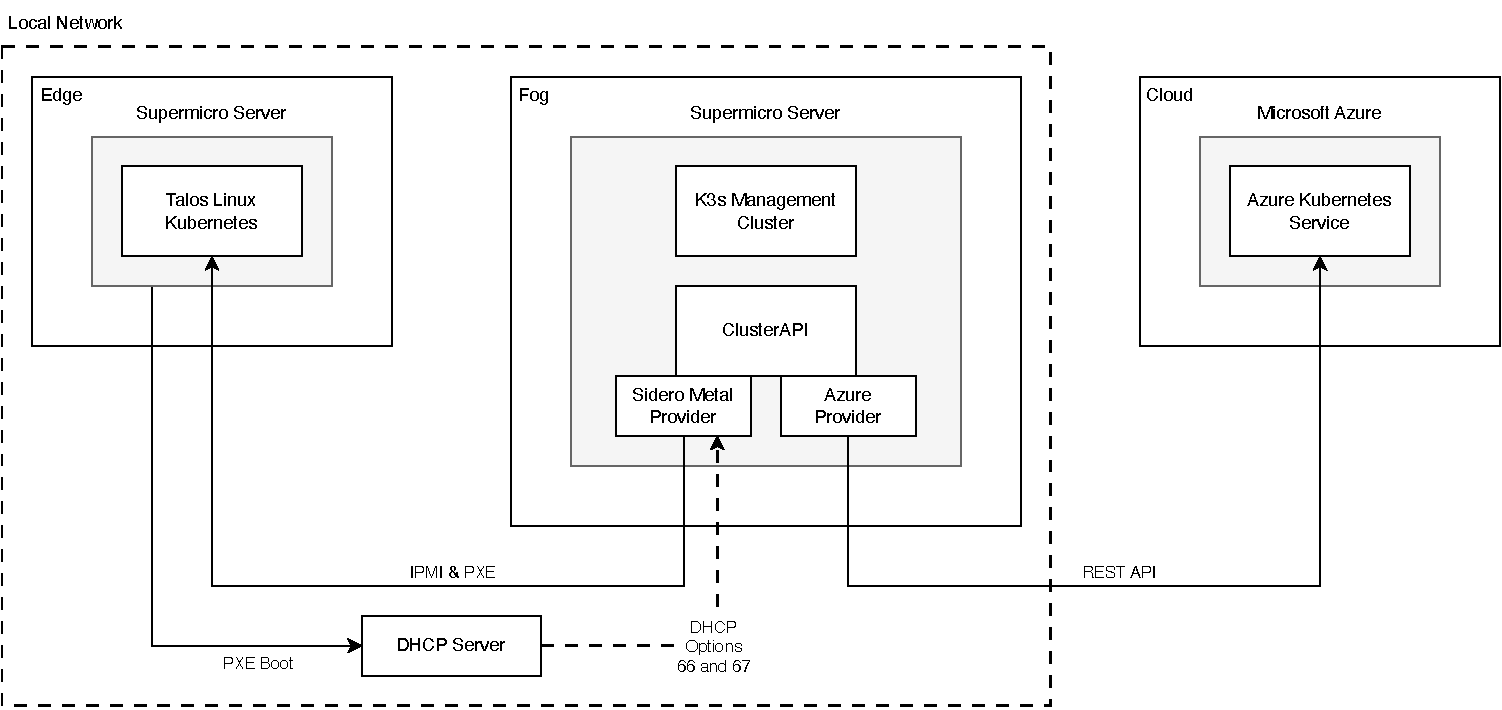
\includegraphics[width=\textwidth]{img/provisioning-infrastructure.pdf}
            \caption{Infrastructure Provisioning with ClusterAPI}
            \label{figure:capi-infra-provisioning}
        \end{figure}

        \autoref{figure:capi-infra-provisioning} illustrates how the provisioning of infrastructure was set up in the project. The management cluster (center), which in this setup was placed in the fog environment, provisioned a managed ``Azure Kubernetes Service'' (AKS) in the Microsoft Azure cloud using the ClusterAPI Provider Azure, which is all there was to the infrastructure provisioning in the cloud environment. Within the local network section, which resembled the on-premises setup in a production site, the Sidero Metal ClusterAPI provider started to provision an edge device, which in practice was a Supermicro bare-metal server, by instructing it to boot via the IPMI. During the boot, the Supermicro server started to initiate the PXE boot process (see \autoref{subsection:network-boot}) during which a broadcast request was sent to the local network and finally received by the DHCP server. The DHCP server had the DHCP options 66 (IP address) and 67 (boot file name) pointed at the Sidero Metal ClusterAPI provider component that held the PXE-relevant files and answered with a boot offer. With these options, the edge device could boot into the operating system and could then finally be provisioned with Kubernetes. We now had a system that was capable of provisioning Kubernetes instances both in cloud providers and onto bare-metal machines. 

    \section{GitOps Setup}
    \label{section:gitops-poc-setup}
        
        Since we discovered how GitOps is essential for a modern IIoT system of scale when following the reference architecture described in this work in \autoref{section:architecture-gitops}, we needed to embed the framework into this multicluster setup. The most common GitOps controllers in the market are FluxCD and ArgoCD and are both fully capable of fulfilling the requirements for this system. In our proof-of-concept setup, we chose FluxCD due to its lightweight and straightforward setup, along with its seamless integration with Mozilla SOPS for secret management (see \autoref{subsection:secret-management-tools-poc}).\newline

        To be able to sustain the GitOps setup at scale we started by setting up the structure of the Git repository for the GitOps-relevant folders. Inspired by the open-source project ``Das Schiff'' by the ``Deutsche Telekom Technik'', which is a GitOps-based Kubernetes Cluster-as-a-Service platform, we created the directory ``cluster-definitions'', which held all GitOps-related configurations like which paths from which repository to reconcile, and the directory ``cluster-components'' which contained the components that should be deployed onto the clusters \cite{telekom_dasschiff}. Both of these folders contained one subfolder per cluster in our setup, but any kind of folder structure would have been possible here. In the cluster-components directory, we also added a ``shared'' folder that held manifests that could be reused by different clusters like the deployment of a dashboard for the FluxCD GitOps controllers.

        Once the structure was set up, we continued by setting up FluxCD on the management cluster. To begin with, we created a Kubernetes secret containing a GitHub token, that enabled FluxCD to access our private GitHub repository, and stored it in Git as an encrypted file using the secret management tool Mozilla SOPS (see \autoref{subsection:secret-management-tools-poc}). As a one-time manual step, we now had to create this secret within the Kubernetes cluster and then install FluxCD manually in order to reach the now fully automated state. Both the secret and the FluxCD installation on the management cluster were now managed by Flux itself through manifests stored in Git. The GitOps controller on the management cluster was now configured to continuously reconcile the specified resources from Git. These resources also contained the ClusterAPI manifests, which then triggered the provisioning of the workload clusters in all environments (see \autoref{subsection:capi}). Once the clusters were provisioned, FluxCD was pushed onto all workload clusters automatically using the FluxCD-specific custom resource ``HelmChartProxy'' which provides the option to install and manage a helm release in a different Kubernetes cluster. An alternative would have been to use the custom resource ``HelmRelease'' which allows to create and manage a helm release and also provides the option to specify a Kubeconfig that determines the target Kubernetes cluster for the deployment of the helm release. This however would have resulted in duplication, since the HelmRelease custom resource has to be created for each workload cluster separately, compared to the HelmChartProxy custom resource that only had to be created once. From then on the GitOps controllers running on the workload clusters continuously reconciled the desired state for the according environment from Git. Together with the secret distribution of secrets like the GitHub token described in the upcoming \autoref{subsection:secret-distribution-strategy}, this resulted in a fully automated infrastructure that resembled the desired infrastructure state of the reference architecture in \autoref{chapter:architecture-proposal}.
        
    \section{Secret Management and Distribution}

        Proper secret management techniques are required in practically every software project, and IIoT platform projects are no different. For this project, we needed to choose a strategy that fits nicely into both the GitOps-driven continuous delivery approach and the multicluster setup due to the high amount of environments. 

        \subsection{Management Tools}
        \label{subsection:secret-management-tools-poc}
        
            To begin with, proper tooling for managing secrets in the project had to be chosen. The following tools are some that allow to declaratively and securely store secrets in an encrypted manner in Git thus allowing to follow the GitOps approach:
    
            \begin{itemize}
                \item Sealed Secrets
                \item External Secrets Operator
                \item Secrets Store CSI Driver
                \item Mozilla Secrets OPerationS (SOPS)
            \end{itemize}
    
            \noindent The tools ``Sealed Secrets'', ``External Secrets Operator'' and ``Secrets Store CSI Driver'' all operate similarly. All of them require the installation of the application and custom resource definitions in the Kubernetes cluster. Instead of then storing the Kubernetes-manifests for secrets in Git directly, developers will create and store instances of the according custom resource definitions. With Sealed Secrets, a developer will encrypt a secret manifest into a ``SealedSecret'' custom resource using a command line interface that interacts with a custom controller running in Kubernetes, which is then safe to store in Git. The custom controller running in the Kubernetes cluster will from then on be the only entity that can decrypt the SealedSecret and will create a Kubernetes secret from it \cite{sealedsecrets}. When using the External Secrets Operator, developers will create manifests that reference secrets in external sources rather than storing encrypted secrets. The custom controller running in the target Kubernetes cluster will fetch the secrets from external sources like AWS Secrets Manager, HashiCorp Vault, Google Secrets Manager, Azure Key Vault and many more and synchronize them into Kubernetes secrets again \cite{externalsecretsoperator}. Similar to that, the Secrets Store CSI Driver references secrets from external sources. While also being capable of syncing the external secrets to Kubernetes secrets, its main intent is to directly mount secrets from an external source into the file system of Kubernetes pods as volumes. This method can improve security by directly mounting secrets as volumes instead of storing them in etcd. Since secrets in Kubernetes are merely encoded using base64 and thus remain readable to anybody with access. In contrast with mounting the secret directly as a volume, the exposure of sensitive data and its potential attack surface is minimized \cite{secrets-csi-driver}. \newline
    
            Being able to remain operational during network disruptions is essential for IIoT systems, especially in on-premises environments in manufacturing sites. This is why we ruled out the External Secrets Operator and the Secrets Store CSI Driver, since they both mainly rely on external sources that require internet access. While integrations to self-hosted secret management systems like HashiCorp Vault, which would enable the tools for offline use, exist, we did not have such a system in use. The final decision between using Sealed Secrets and Mozilla SOPS mainly revolved around flexibility. While Sealed Secrets is easy to use and integrates seamlessly into Kubernetes, it is limited to secrets in Kubernetes. Mozilla SOPS on the other hand is a tool that only encrypts and decrypts files using a variety of encryption mechanisms like Azure Key Vault, age or PGP making them safe to store in Git. Given its versatility beyond Kubernetes, SOPS can serve as a unified secret management tool for all project-related secrets, accommodating not only Kubernetes deployments but also those used directly in scripts and other non-Kubernetes applications \cite{mozillasops}. Mozilla SOPS also provides simple integrations with common GitOps controllers like ArgoCD and Flux, as already mentioned in \autoref{section:gitops-poc-setup}. While we chose to use Mozilla SOPS in this project, a solution for different projects must be chosen based on the requirements of the project in question.

        \subsection{Multicluster Strategy}
        \label{subsection:secret-distribution-strategy}

            With SOPS as the secret management solution in place, we needed a strategy for managing and distributing secrets in all environments across the IIoT system. Since such a system, especially at scale, involves many different parties or even tenants, it is essential that access to confidential secrets is scoped according to the principle of least privilege which might for example mean that each team working on the project is only able to decrypt its own secrets. In this PoC project, we decided that each instance of each environment should have a designated encryption key to demonstrate this. When creating a new environment, in particular the Kubernetes cluster, we created a new GPG key. While this was only required a single time per new environment instance, it was still manual work that might become tedious at scale. How this can be automated will be discussed in the further work in \autoref{section:further-work}. Using this key, developers could now encrypt (and decrypt) secrets relevant to this environment and store them in a Git repository safely, without others with access to the repository being able to decrypt it again. The platform team that managed the whole IIoT system had its own SOPS key, which in practice was a key in the Azure Key Vault. Using this key, all GPG keys of the teams were encrypted again, in order to be able to safely store these in Git as well. \newline
            
            Using a ``ClusterResourceSet'', which is a custom resource of the ClusterAPI project (see \autoref{subsection:capi}) that allows to apply a set of resources defined by users to the workload clusters, the GPG keys were distributed to the according environments as Kubernetes secrets. An alternative to the ClusterResourceSet, which is still marked as an alpha version, would have been using the feature set of the GitOps controller. Both FluxCD and ArgoCD support specifying a custom Kubeconfig (``destination'' in ArgoCD) for reconciling resources, thus enabling the platform team to push the GPG key secrets from the management cluster to the workload clusters. In this project, we used the approach with the ClusterResourceSet custom resource, since at the time of setting up the PoC we were not aware of the option to use the GitOps controller directly. 
            
            Once the GPG keys were created as secrets in the environments, teams could now retrieve their GPG keys for encrypting and decrypting their secrets. Also, the GitOps controllers running in each environment could use this GPG key for decrypting secrets relevant to that environment. In this setup, each environment had a folder called ``secrets'' in its respective cluster-components folder (see \autoref{section:gitops-poc-setup}). The GitOps controller was then instructed to reconcile this folder by decoding the manifests using the environment-specific GPG key which was now present as a Kubernetes secret. This setup was not only useful for the distribution of GPG keys or the use of environment-specific secrets however. By using the option to push secrets from the central management cluster to practically all workload clusters, we could easily distribute secrets required in all environments like the credentials to our observability components as further discussed in \autoref{section:observability}, which simplified operational tasks regarding secrets and credentials immensely.\newline

            This approach worked nicely in practice and offered a flexible, scalable and secure strategy for managing secrets in a multicluster setup. For real projects, using the GitOps controller for distributing secrets seems like the better and more robust choice compared to using the ClusterResourceSet custom resource from ClusterAPI which is still in alpha. Since SOPS allows to encrypt a file with multiple keys, it also proved to be useful to add the key of the platform team to critical secrets of teams to be able to support them with their secret management during development.
    

    \section{Observability}
    \label{section:observability-poc-setup}

        As we discovered the importance of having proper observability across a software system in \autoref{section:observability}, we needed to set up tooling for metrics and logs within the system.\newline

        \begin{figure}[htbp]
            \centering
            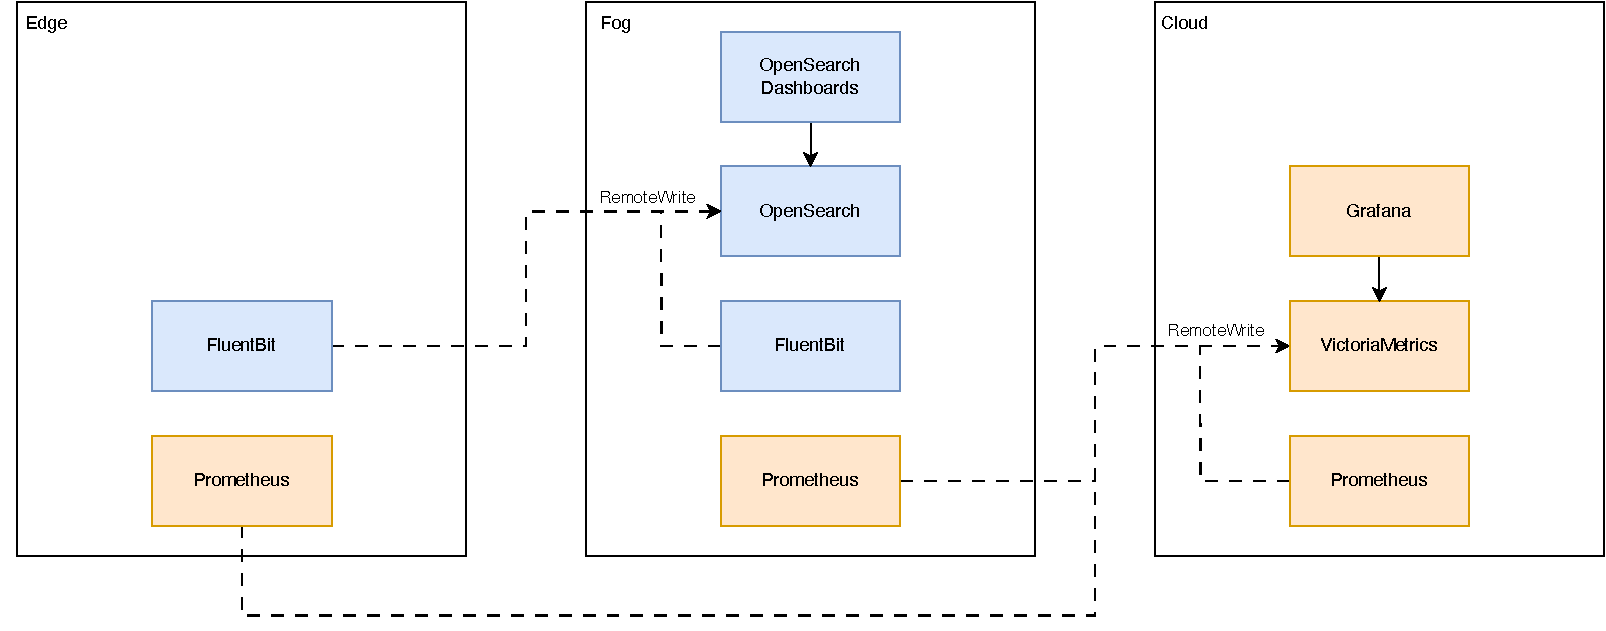
\includegraphics[width=\textwidth]{img/observability.pdf}
            \caption{Multicluster Observability}
            \label{figure:observability}
        \end{figure}

        \noindent To record metrics, we started by deploying a Prometheus instance onto each cluster in the system. Prometheus is an open-source database optimized for time series data that supports scraping and storing metrics from various sources. These Prometheus instances then gathered metrics for the according environment and acted as buffers by storing them locally. These buffers reduced the risk of losing metrics due to downtimes or network disruptions. The reference architecture suggests having a centralized cloud-based metric store across the whole IIoT system, which is why we deployed an instance of VictoriaMetrics in the cloud environment. VictoriaMetrics is an open-source project that offers similar functionality and identical APIs to Prometheus but solves common problems of Prometheus like the struggle with long-term storage and the lack of support for remote writes from remote Prometheus instances \cite{victoriametrics}. Suitable alternatives include Grafana Mimir, Thanos or InfluxDB. To accumulate metrics across the whole system, each Prometheus ``buffer'' instance was configured to remotely write its data into the VictoriaMetrics instance in the cloud for long-term storage as \autoref{figure:observability} illustrates with the dotted lines between the orange components. The open-source analytics and monitoring solution Grafana was used to visualize the metrics across the whole system in one centralized location. \newline

        For logging, the reference architecture recommends only aggregating logs per production site due to the volume of the data. To achieve this, the open-source search engine ``OpenSearch'' was deployed once per production site. OpenSearch is scalable and supports high availability, making it a well-suited storage solution for centralized logging. Alternatives encompass ElasticSearch, Grafana Loki or Apache Solr. For shipping logs from all servers in the production site into the search engine, the log shipper ``FluentBit'' was used. It was deployed on each Kubernetes node using a Kubernetes DaemonSet and ingested the logs from the according nodes into OpenSearch for persistent storage, as the dotted lines between the blue components in \autoref{figure:observability} display. FluentBit also enriched the logs by adding metadata like the name of the pod or even the cluster in which the logs occurred to the logs, to increase their value even further. Lastly the open-source tool ``OpenSearch Dashboards'' was used as a graphical user interface for visualizing and querying the log data stored in OpenSearch. 
    

    \section{Multicluster Management}

        In \autoref{section:multicluster-mgmt} we described how a multicluster management solution can be beneficial. While we already decided to use ClusterAPI for the provisioning of clusters and their operation, tools like the Enterprise Kubernetes Management Platform ``Rancher'' or the enterprise product ``D2iQ Kubernetes Management Platform - DKP'' could still add valuable functionality like centralized management of role-based access across all environments or access to all clusters from a single location through network tunnels. In this PoC we deployed the Rancher platform by simply adding a ``HelmRelease'' using FluxCD to the management cluster. The provided functionality worked nicely and is essential to have once the system grows beyond a few environments.

        However, we soon discovered that Rancher did not yet support a fully declarative GitOps setup at the time of writing this work. Onboarding a workload cluster into Rancher management could be initiated by applying a custom resource ``Cluster'' into the management cluster. Once the custom object was applied, the ``Rancher Agent'', which connects to the Rancher platform, had to be applied to the workload cluster. For this, Rancher provided the necessary deployments as YAML manifests via an endpoint, but only after having registered the new cluster. While these manifests could again be stored in Git in the according folders of the workload cluster, this manual step of fetching the dynamically generated manifests broke the GitOps workflow. Also, if an already onboarded workload cluster would ever get recreated from scratch this whole onboarding process would have to be repeated. Since the multicluster management solution still provided valuable features, this manual work was accepted for this PoC project however. A strategy on how to deal with this issue in a real project is described in \autoref{section:further-work}.


    \section{Unified Namespace Implementation}

        At this point, the necessary platform infrastructure was in place for the actual IIoT infrastructure services to be deployed. Since this work focuses on the infrastructure, the last thing to do was to set up the unified namespace described in \autoref{section:unified-namespace}. 

        As a first step, we deployed the MQTT broker in the cloud environment. While any broker fully compatible with the MQTT 5 standard could have been chosen here, we decided to use the HiveMQ MQTT broker. For deploying a production-grade broker in the cloud on Kubernetes, we used the official HiveMQ Kubernetes Operator that helps orchestrate and manage the lifecycle of a highly available HiveMQ cluster. Not only does the operator deploy HiveMQ, but it also assists in monitoring, maintaining, recovering, and upgrading HiveMQ during the operation \cite{hivemq_operator}. All of this was achieved by simply adding manifests, mainly using the FluxCD's ``HelmRelease'' custom resource, to the corresponding directories in Git.
        
        Moving forward we needed to deploy an MQTT broker in each production site, i.e.\ the Kubernetes cluster in each fog environment. For this, we used the recently released HiveMQ Edge broker. Not only is this broker optimized for edge environments due to lower resource requirements, but it also helps to set up a unified namespace by providing plug-and-play integrations with common OT protocols like Modbus and OPC-UA. This means that we no longer needed to deploy custom adapter services for these integrations \cite{hivemq_edge_website}. This broker was also simply deployed by adding manifests to Git and letting the GitOps controller reconcile it eventually. Through custom configuration, the HiveMQ Edge broker was instructed to set up a bidirectional MQTT bridge between the on-premises and cloud brokers by publishing all messages on all topics to and subscribing to all relevant topics from the cloud broker. As a last step, we deployed several NodeRED instances in the edge environment. NodeRED is a browser-based low-code programming tool that is often used by developers to quickly set up IoT applications. In our case, we used NodeRED to simulate edge devices that publish data into the unified namespace via the on-premises MQTT broker. An example topic used for this was ``enterprise-1/site-1/area-1/line-1/cell-1'' (see \autoref{section:unified-namespace}). Note that in this setup security concerns like proper IP whitelisting and RBAC were not dealt with since this project was only meant to be a proof-of-concept. 

        \begin{figure}[htbp]
            \centering
            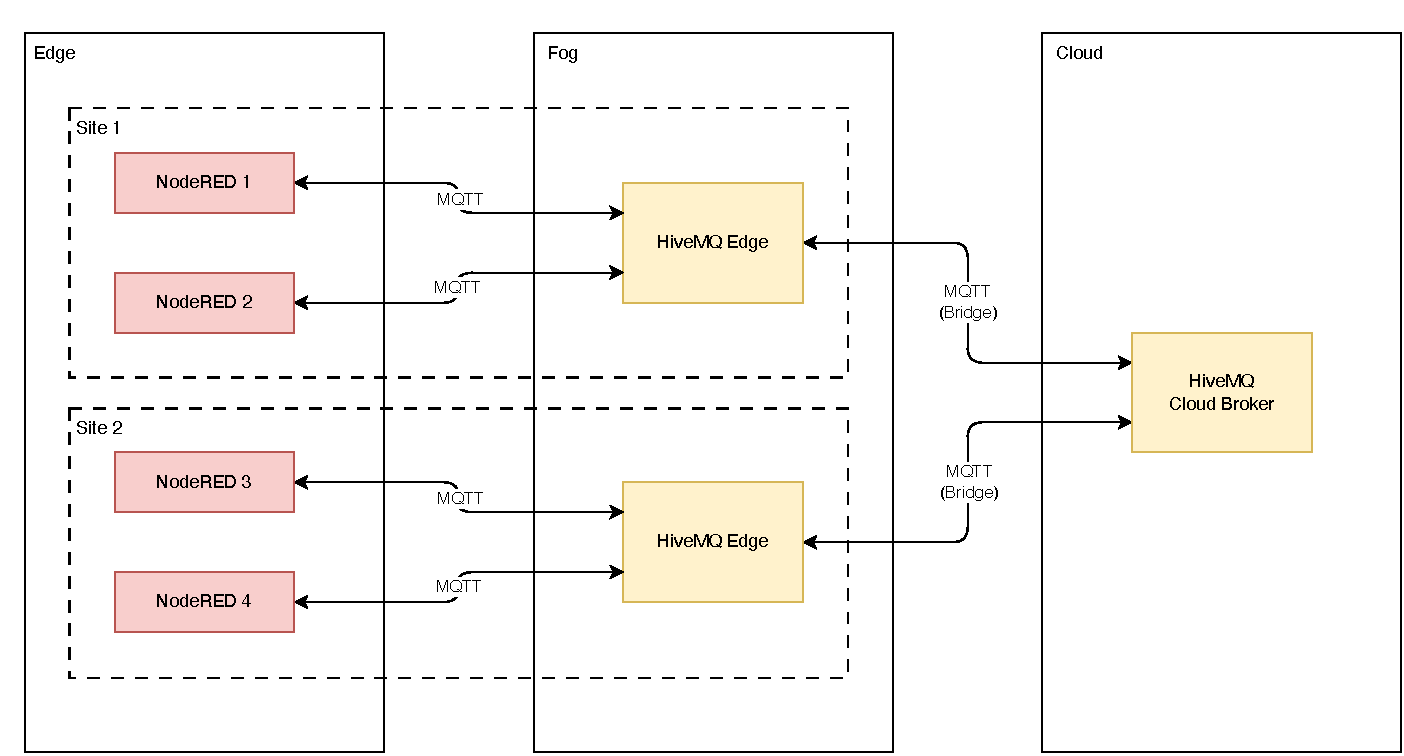
\includegraphics[width=\textwidth]{img/uns-poc.pdf}
            \caption{Unified Namespace Implementation}
            \label{figure:uns-poc}
        \end{figure}

        \noindent \autoref{figure:uns-poc} illustrates how this unified namespace setup could now be scaled to any number of edge devices and production sites. Each IIoT component, in this case, the NodeRED instance, in the edge environments could bidirectionally communicate with the on-premises HiveMQ Edge broker. Workloads in the edge or fog environment were able to access the on-site data with low latency by subscribing to the edge broker directly. Use cases like long-term storage or stream analytics that require high amounts of computational power or storage could be realized in the cloud environment.


    \section{Implementation Review}
        The implementation of the reference architecture in this proof-of-concept resulted in an extensible, scalable, flexible and robust system. Deploying, decommissioning, or moving workloads around the whole system was simple and the onboarding of (simulated) IIoT devices into the unified namespace in an on-premises environment was a smooth process.

        Using ClusterAPI to provision Kubernetes instances onto various kinds of infrastructure proved to be a solid and powerful choice. The bare-metal infrastructure provider Sidero Metal was easy to work with and made provisioning onto plain hardware an easy task. It is possible that using the CNCF project Metal$^3$ in favor of Sidero Metal would be beneficial for real-world projects since it uses the battle-tested OpenStack Ironic for hardware management and thus is capable of managing a wider variety of infrastructure in a more robust manner. However since Sidero Metal supports both PXE and IPMI which was required for the hardware in use, it was a reasonable choice for this proof-of-concept. It has to be mentioned that using out-of-band management techniques and network boot for provisioning hardware is a strategy that can fail at many points, and can be simplified immensely by employing virtualization e.g.\ using VMware vSphere which offers stable and reliable APIs for managing virtual machines at the cost of a small loss in performance (see \autoref{section:virtualization}).

        The use of the GitOps framework also showed great results. Having a continuous versioning mechanism in the single source of truth for the whole infrastructure was very useful, especially during development. Also having the option of applying a Git workflow with pull requests and code reviews felt like a great basis for a large-scale project. The GitOps controller ``FluxCD'' worked nicely and did not show any unexpected behavior. Together with the observability stack, which provided comprehensive monitoring and logging capabilities across all components of the IIoT platform, the integration of FluxCD within the GitOps framework greatly enhanced our overall infrastructure management.

        Lastly, the multicluster management solution Rancher proved to be a useful tool. Even though it was not used for provisioning clusters in this setup, the remaining feature set was a meaningful addition to the management capabilities across such a large-scale system. As Rancher does not yet offer full support for the GitOps model, it is necessary to assess each project individually to determine whether developing custom software for integrating Rancher into the GitOps framework is advisable (see \autoref{section:further-work}). Alternatively, one could consider either manually onboarding clusters into Rancher or opting for a different multicluster management solution.

